\documentclass[12pt]{extarticle}
\usepackage{tempora}
\usepackage[T1, T2A]{fontenc}
\usepackage[utf8]{inputenc}
\usepackage[english, ukrainian]{babel}
\usepackage{geometry}
\usepackage{graphicx}
\usepackage{multirow}
\usepackage{multicol}
\usepackage{float}
\graphicspath{{/home/artem/Pictures}}
\geometry
{
    a4paper,
    left=30mm,
    top=15mm,
    right=20mm,
    bottom=15mm,
}

\begin{document}
\begin{titlepage}
    \begin{center}
        \textbf{\normalsize{\MakeUppercase{
            Міністерство Освіти і науки України
            Національний університет "Львівська політехніка"
        }}}

        \begin{flushright}
        \textbf{ІКНІ}\\
        Кафедра \textbf{ПЗ}
        \end{flushright}
        \vspace{15mm}

        \includegraphics[width=0.4\textwidth]{lpnu_logo.png}

        \vspace*{\fill}

        \textbf{\normalsize{\MakeUppercase{Звіт}}}
            
        До лабораторної роботи №4

        \textbf{на тему:} “ Метод сортування злиттям.”

        \textbf{з дисципліни:} "Алгоритми і структури даних”
            
        \vspace*{\fill}

        \begin{flushright}

            \textbf{Лектор:}\\
            доцент кафедри ПЗ\\
            Коротєєва Т. О.\\
            \vspace{12pt}

            \textbf{Виконав:}\\
            студент групи ПЗ-24\\
            Губик А. С.\\
            \vspace{12pt}

            \textbf{Прийняв:}\\
            асистент кафедри ПЗ\\
            Вишневський К. О.\\
        \vspace{12pt}
        \end{flushright}

        Львів -- 2023
            
            
    \end{center}
\end{titlepage}

\subsection*{Тема роботи} 
Метод сортування злиттям.

\subsection*{Мета роботи} Вивчити алгоритм сортування злиттям. Здійснити програмну реалізацію алгоритму сортування злиттям. Дослідити швидкодію алгоритму сортування злиттям.

\subsection*{Індивідуальне завдання } 
Варіант 6:
Задано одномірний масив дійсних чисел. До від’ємних елементів масиву застосувати функцію $\sin x$ . Отриманий масив посортувати в порядку спадання.


\subsection*{Теоретичні відомості}
Сортування злиттям (англійською «Merge Sort») — алгоритм сортування, в основі якого лежить принцип «розділяй та володарюй» (англійською «Divide and Conquer»). В основі цього способу сортування лежить злиття двох упорядкованих ділянок масиву в одну впорядковану ділянку іншого масиву.

Під час сортування в дві допоміжні черги з основної поміщаються перші дві відсортовані підпослідовності, які потім зливаються в одну і результат записується в тимчасову чергу. Потім з основної черги беруться наступні дві відсортовані підпослідовності і так до тих пір доки основна черга не стане порожньою. Після цього послідовність з тимчасової черги переміщається в основну чергу. І знову продовжується сортування злиттям двох відсортованих підпослідовностей. Сортування триватиме до тих пір поки довжина відсортованої підпослідовності не стане рівною довжині самої послідовності.

Сортування злиттям можна задати рекурсивно: масив поділяється на дві приблизно рівні частини, які після сортування (тим самим способом) зливаються. Коли ж довжина частини масиву зменшується до 1, відбувається повернення з рекурсії. Завершуючи описання сортування злиттям, скажемо, що цей алгоритм є першим із ефективних алгоритмів сортування. У 1945 році його винайшов Джон фон Нейман, один із піонерів програмування.

Час роботи алгоритму T(n) по впорядкуванню n елементів задовільняє рекурентному співвідношенню: T(n) = 2T(n/2) + O(n), деT(n/2) — час на впорядкування половини масиву, O(n) — час на злиття цих половинок.

Враховуючи, що T(1) = O(1), розв’язком співвідношення є: T(n) = O(nlog(n)).

Крім того, алгоритм потребує для своєї роботи E(n) додаткової пам’яті.

Алгоритм не міняє порядок розташування однакових елементів, а отже він є стабільним.

Швидкість алгоритму є асимптотично оптимальною. Але її можна пришвидшити в константну кількість разів.Можливі оптимізаці:

Оптимізація впорядкування невеликих частин масиву — невеликі частини масиву (наприклад, при n < 50) впорядковувати сортуванням вставкою.
Оптимізація кількості копіювань елементів — при злитті двох впорядкованих масивів в один, кожен елемент копіюється два рази (спочатку у тимчасовий масив, а потім знову у початковий). Кількість копіювань можна зменшити удвічі, якщо по черзі використовувати для об’єднання початковий і тимчасовий масиви. Тоді можна не виконувати зайві операції копіювання.
\subsection*{Покроковий опис}

\begin{enumerate}
\item \textbf{Функція:} До від'ємних елементів застосовуємо $\sin x$ 

\item \textbf{Розбиття:} Початковий масив 
розділяється навпіл, утворюючи два підмасиви.
\item \textbf{Сортування:} Кожен з цих підмасивів 
рекурсивно сортується за допомогою того ж алгоритму сортування злиттям.
\item \textbf{Злиття :} Вже відсортовані підмасиви
 об'єднуються в один великий відсортований масив. Під час об'єднання елементи порівнюються і зливаються в правильному порядку.

\end{enumerate}

\subsection*{Вихідний код}

{\fontfamily{pcr}\selectfont

\begin{verbatim}
#include <iostream>
#include <vector>
#include <cstdlib>
#include <ctime>
#include <algorithm>
#include <cmath>
#include <chrono>

// Merge function for merge sort
void merge(std::vector<float>& arr, int left, int middle, int right) {
        static int step = 1;
        int n1 = middle - left + 1;
        int n2 = right - middle;

        std::vector<float> leftArr(n1);
        std::vector<float> rightArr(n2);

        for (int i = 0; i < n1; i++) {
                leftArr[i] = arr[left + i];
            }
        for (int j = 0; j < n2; j++) {
                rightArr[j] = arr[middle + 1 + j];
            }

        int i = 0, j = 0, k = left;
        while (i < n1 && j < n2) {
                if (leftArr[i] <= rightArr[j]) {
                        arr[k++] = leftArr[i++];
                    } else {
                        arr[k++] = rightArr[j++];
                    }
            }

        while (i < n1) {
                arr[k++] = leftArr[i++];
            }

        while (j < n2) {
                arr[k++] = rightArr[j++];
            }
        std::cout << "Step" << step << ": ";
        for (const float& num : arr) {
                std::cout << num << " ";
            }
        std::cout << std::endl;
        step++;
    }

// Merge Sort function
void mergeSort(std::vector<float>& arr, int left, int right) {
        if (left < right) {
                int middle = left + (right - left) / 2;

                mergeSort(arr, left, middle);
                mergeSort(arr, middle + 1, right);

                merge(arr, left, middle, right);
            }
    }

int main() {
        // Seed the random number generator
        std::srand(static_cast<unsigned>(std::time(nullptr)));

        // Get the size of the vector from the user
        int vectorSize;
        std::cout << "Enter the size of the vector: ";
        std::cin >> vectorSize;

        // Generate a vector of random float numbers between 0 and 100
        std::vector<float> numbers;
        for (int i = 0; i < vectorSize; i++) {
                float randomFloat = static_cast<float>(std::rand()) / static_cast<float>(RAND_MAX);
                // Scale the random number to the range [-100, 100]
                randomFloat = randomFloat * 200.0f - 100;
                numbers.push_back(randomFloat);
            }

        for (float& num : numbers) {
                if (num < 0) {
                        num = std::sin(num);
                    }
            }


        std::cout << "Unsorted Vector:" << std::endl;
        for (const float& num : numbers) {
                std::cout << num << " ";
            }
        std::cout << std::endl;

        // Measure sorting time
        auto startTime = std::chrono::high_resolution_clock::now();

        // Merge Sort the vector
        mergeSort(numbers, 0, numbers.size() - 1);

        auto endTime = std::chrono::high_resolution_clock::now();
        auto duration = std::chrono::duration_cast<std::chrono::nanoseconds>(endTime - startTime);

        // Apply sin function to negative elements
        // Print the modified vector
        std::cout << "Modified Vector:" << std::endl;
        for (const float& num : numbers) {
                std::cout << num << " ";
            }
        std::cout << std::endl;

        std::cout << "Sorting time: " << duration.count() << " nanoseconds" << std::endl;

        return 0;
    }


\end{verbatim}
}
\vspace{12pt}
\begin{figure}[H]
    \centering
    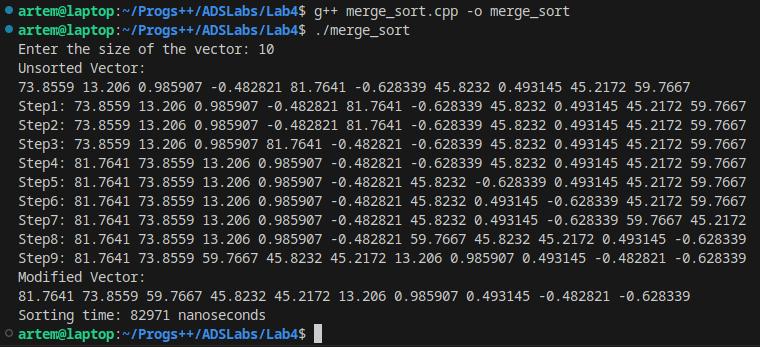
\includegraphics[width=0.90\textwidth]{Screenshot_20231018_002440.png}
    \caption{}
\end{figure}
\subsection*{Висновок} 
Сортування злиттям - це ефективний алгоритм, який завжди має часову складність O(n * log(n)), де n -- кількість елементів у масиві.
\end{document}
